\documentclass[12pt,a4paper,oneside]{article}
\usepackage{graphicx}
\usepackage{float} %for [H]


\usepackage{titlepic}
\usepackage[utf8]{inputenc}
\usepackage[left=1.1in,right=1.1in, top=1in, bottom= 1in]{geometry}
\usepackage[none]{hyphenat} % Avoids to go out of margin
\usepackage{subfiles}

% Font size of figure smaller than normal size:
\usepackage{caption}
\captionsetup[figure]{font=small}
\linespread{1.2}

% --------------------------------------------- %

\title{Homework 2}	                                    % Title
\author{Flavio Maiorana 2051396}				        % Authors separated by \\
\date{\today}								            % Date

\makeatletter
\let\thetitle\@title
\let\theauthor\@author
\let\thedate\@date
\makeatother

\begin{document}

\begin{titlepage}
	\centering
    \vspace*{0.5 cm}
    
\includegraphics[scale = 0.75]{figures/SapienzaLogo.pdf}\\[1.0 cm]	% University Logo

    % \vspace*{-0.4cm}
    % \textsc{\large DIAG}\\[2.0 cm]	% Department Name
    % \vspace*{1cm}

    { \fontsize{20.74pt}{18.5pt}\selectfont\bfseries \thetitle \par } % Title

    \vspace*{0.25cm}
    \textsc{\Large Machine Learning}\\[0.5 cm] % Course Name

    \vspace*{2.6cm}
	% \begin{minipage}{0.4\textwidth} % 0.4
	% 	\begin{flushleft} \large
	% 		\textbf{Professors:}\\
	% 		Professor Name\\
	% 	\end{flushleft}
	% \end{minipage}~
	\begin{minipage}{0.3\textwidth} %0.4
		\begin{flushright} \large
		\begin{minipage}{1\textwidth}
		\begin{flushleft} \large
			\textbf{Students:} \\
			\theauthor
        \end{flushleft}
        \end{minipage}
		\end{flushright}
	\end{minipage}\\[3.85 cm]

    \vspace{2cm}
    \rule{\linewidth}{0.2 mm} \\[0.3 cm]
    \vspace*{-0.2cm}
    Academic Year 2023/2024
\end{titlepage}
\newpage

\section{Introduction}

First of all, it could be useful to gain some insight one how the dataaset is
made. The available data is already split into training and testing set. We
will consider the test split only in the evaluation phase (to prevent
data leakage).

\begin{verbatim}[Dataset for Training]
    N Examples: 6369
    N Classes: 5
    Classes: [0 1 2 3 4]
    - Class 0: 1000 (15.701051970482022)
    - Class 1: 1500 (23.551577955723033)
    - Class 2: 1500 (23.551577955723033)
    - Class 3: 2000 (31.402103940964043)
    - Class 4: 369 (5.7936881771078665)
\end{verbatim}

Some comments: the dataset is highly imbalanced. That needs to be addressed
accordingly. The main two problems to address are:

\begin{itemize}
    \item Model architecture
    \item Training process
    \begin{itemize}
        \item Class imbalance mitigation
        \item Optimization choice
    \end{itemize}
\end{itemize}

Before everything else, it is worth to mention the performance metrics. Since
the dataset is highly imbalanced, accuracy might not be the best choice to
measure performance. Rather, the weighted mean of f1-scores (and also recall and
precision) could be a better choice. 

\section{Training process}

There are some important issues to address, which are to some extent independent
from the model we use to classify. First of all, to mitigate class imbalance we
could apply:
\begin{itemize}
    \item Data augmentation (useful in any case to increase generalization)
    \item Different sampling techniques
    \begin{itemize}
        \item Upsampling/Downsampling
        \item Weighted resampling
    \end{itemize}
\end{itemize}

\subsection{Sampling techniques}

Different sampling of data in order to rebalance the classes. These techniques
use also data augmentation techniques, in order to make the network as
generalizing as possible. Data augmentation is used obviously also without
resampling techniques.

\subsection{Data augmentation}

This technique is widely used with images. It exploits the invariance property
of images to enhance generalization properties of neural networks. In our case
it is particularly useful, because it allows us to "reuse" the same sample
multiple times and make it look new to the network by augmenting its features.
The transformation I used are these three from the torchvision package, plus a
random color jitter implemented separately. I also tried
RandomHorizontalFlipping, but I noticed actually worse conditions, maybe because
the images are sensitive to the horizontal orientation (for turning left and
right), so randomly flipping them would mean introducing noise to the labels.

\begin{verbatim}
    transforms.RandomInvert(),
    transforms.RandomErasing(),
    transforms.RandomRotation(degrees=5),
\end{verbatim}

\subsubsection{Weighted random resampling}

In order to mitigate class imbalance, one could try to rebalance the dataset by
using weighted resampling techniques. This can be achieved by
torch.data.WeightedRandomSampler. The weights can be chosen according to class
distribution, but I achieved better performance by tuning them 'by hand'. More
in particular, the weights have to be chosen such that every batch has an equal
distribution among all classes. 
\begin{verbatim}
    [0.8,0.6,0.6,0.5,1.7]
\end{verbatim}
For example, after some trials, the above weights vector proved itself to
perform better than withoud weighted resampling. 

Naturally, class 3 has to be sampled with the least probability, and class 4
with the highest probability. Besides, the data will be resampled with
replacement. I was able to reach a satisfactory performance with some manual
tuning of the class weights, but the problem of this approach is that the
weightedsampler is not perfectly reproducible, which means that performance from
one trained model to the other. Nevertheless, I was able to complete the entire
lap only with this method.

\subsubsection{Over/undersampling}

Another useful and potentially effective technique to make up for class
imbalance is over and undersampling. To that end, I used the python package
imblearn, that offers out-of-the-box methods to under/over sample a dataset. I
used the SMOTEENN method, which first oversamples all but the minority class by
'generating' new samples through interpolation between two existing samples.
After that, ENN is applied, which polishes the newly generated samples, removing
the nearest one to each other. After over and under sampling the new dataset
will look like this. We lost some samples, but now the dataset is more balanced
and well distributed.
\begin{verbatim}
    N Examples: 3399
    N Classes: 5
    Classes: [0 1 2 3 4]
    - Class 0: 515 (15.151515151515152)
    - Class 1: 628 (18.476022359517504)
    - Class 2: 658 (19.358634892615477)
    - Class 3: 903 (26.5666372462489)
    - Class 4: 695 (20.44719035010297)
\end{verbatim}

\begin{figure}[H]
    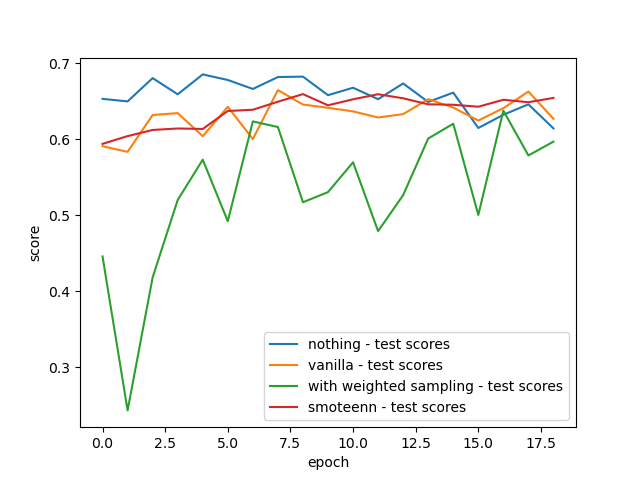
\includegraphics{figures/compare.png}
    \caption{Different methods compared}
\end{figure}

Anytime an image is sampled, these transforms are applied, resulting in a
completely new image.

\subsubsection{Comparing them all}

In the end, from the point of view of the f1-score the performances are all
similar, maybe smoteenn has a slighlty better performance. But in the end, on
the track the method using nothing always behaves badly, the others do better.
The video uses weighted random resampling.

\subsection{Optimizer}

I tested two different optimizers: SGD and Adam. The second one had generally a
better performance, resulting in a smoother optimization process. The best
learning rate was 0.0001. A bigger lr resulted in a 'ripple' effect on the
learning process, due to the 'jumps'.

\subsubsection{Early stopping}
One could also implement a stopping mechanism. That is helpful to stop the loss
from sinking while having a performance measuramente on a validation set, which
means we are overfitting on the training data. The validation split needs to be
totally independent from training data, namely no data augmentation on it.
Regarding early stopping, it is important to adequately choose the 'patience'
parameter. It indicates the number of epochs after which, if the validation
score is getting worse, training will stop. In general, early stopping can be
applied both to validation score and loss. In my case, a patience lower than 3
resulted in too early stopping, and a patience above 10 resulted in sometimes
overfitting. 

\section{Model Architecture}

The first and foremost choice regarding cnn model architecture is surely how
deep it has to be and how big the kernel need to be. Since the images are not
that big, a reasonably small cnn would be enough, since a too deep one would
either overfit on training data, or waste computational resources without
gaining any improved performance. Although, a too small model would not be able
to adequately catch the features of the image. Also, kernels size is very
important. A too big kernel would compromise computational efficiency, but the
size has to be adapted to the tiype of features the convolution needs to to
capture. To corroborate these concepts we will compare some CNNs with a
different number of convolutional layers. 

Each CNN has similar structure: N convolutional layers, each followed by a batch
normalization layer, then an activation fuction and at last a max pooling layer.
After the convolution layers, responsible for extracting features from the
image, the network has some fully connected layers (with the same activation
function as the convolutional layers) at the end, followed by a final dropout layer,
that have as final output a vector of five elements, expressing the score
predicted for each class. 

In the following part, each list entry indicates the dimension for the convolutional
layer (from 1 to N). The kernel size 0 indicates the number of channels of the
input image. This training results are all captured after 20 epochs.

\begin{itemize}
    \item N = 4
    \begin{verbatim}
        'channels': [3,5,15,30,30],
        'kernels': [7,5,5,5],
        'strides': [1,1,1,1],
        'pool_kernels': [2,2,2,2],
        'pool_strides': [2,2,2,2],
        'fc_dims': [120,5],
        'dropout': 0.2
        Training time: 169.67
    \end{verbatim}
    \item N = 6 
    \begin{verbatim}
        'channels': [3,10,16,32,64,64,64],
        'kernels': [5,5,5,3,3,3],
        'strides': [1,1,1,1,1,1],
        'pool_kernels': [2,2,2,2,2,2],
        'pool_strides': [2,1,2,1,2,1],
        'fc_dims': [576,64,5],
        'dropout': 0.2
        Training time: 400.342
    \end{verbatim}
\end{itemize}

\begin{figure}[H]
    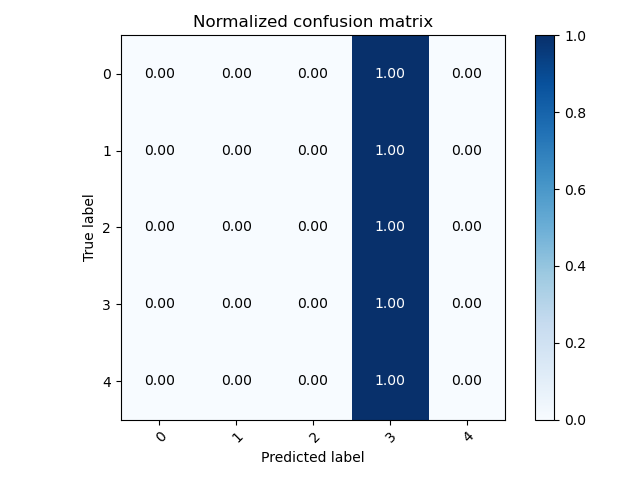
\includegraphics{figures/deeper.png}
    \caption{Deeper network takes more to train and overfits training data}
\end{figure}

\subsection{Dropout layer}

\begin{figure}[H]
    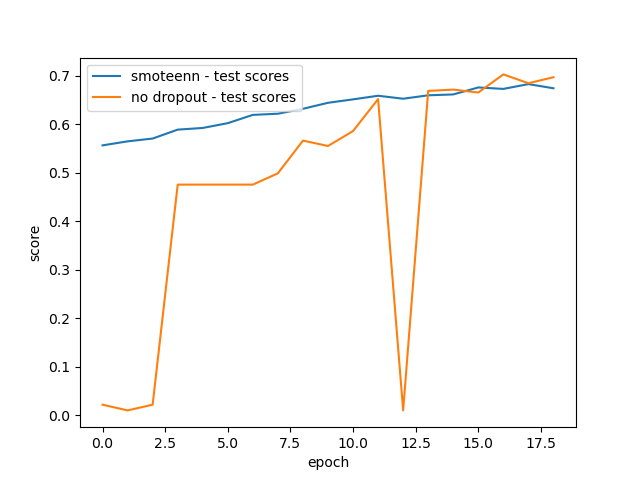
\includegraphics{figures/dropout.png}
    \caption{Dropout}
\end{figure}

This layer is inserted at the end of the fully connected layers. It is
particulary important to avoid overfitting. More specifically, it avoids that
the model overfits too much on training data by inserting some perturbations in
the model, namely by dropping randomly some connections from one layer to the
other. As we can see, with the same exact architecture, just by eliminating the
dropout layer, the learning becomes much different, and so also the result is
different, as we can see from the two confusion matrices.

\begin{figure}[H]
    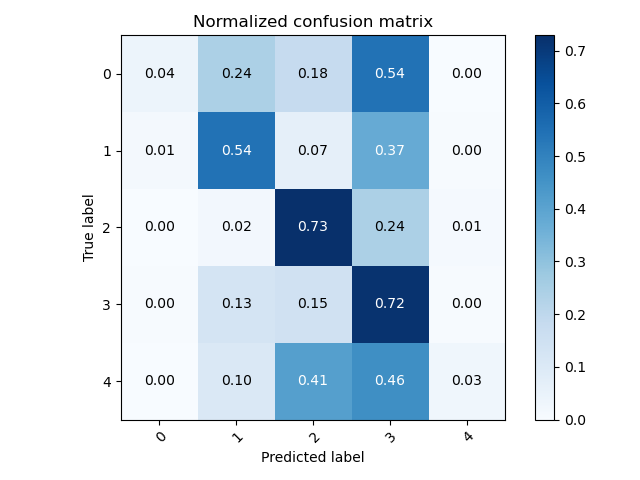
\includegraphics{figures/dropout_confusion.png}
    \caption{Dropout confusion matrix}
\end{figure}

\begin{figure}[H]
    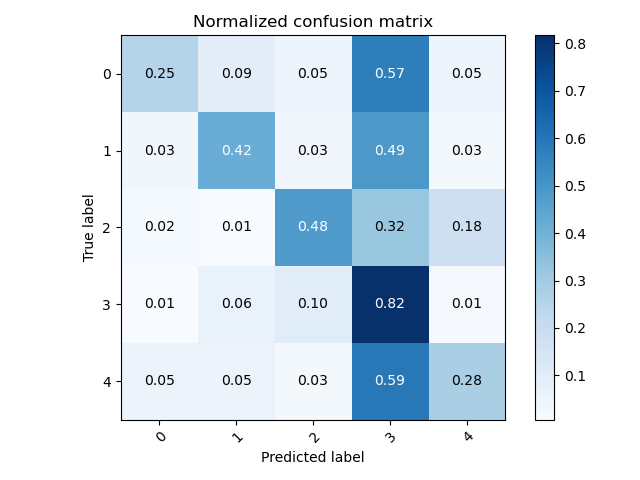
\includegraphics{figures/no_dropout_confusion.png}
    \caption{No Dropout confusion matrix}
\end{figure}

The inference tends more towards class 3, which means overfitting.


\newpage


\section{Final Considerations}

In the end, after different trials I was able to achieve the completion of a
full lap through manual tuning of class weights. The difficulty in this task was
that a relatively high score, whatever the metrics, not always reflected in a
high reward on the real track. Moreover, I noticed that sometimes the car did
better on the track when the model never predicted class 0 or 4, because the
risk is that a false positive of one of these two would stop the car for the
entire episode. So, in general precision needs to be high especially for these
two classes, and that can be regulated better with weighted resampling. 

\bibliographystyle{unsrt}
\bibliography{ref}
\nocite{*}  % to include references which were not cited

\end{document}